\documentclass[12pt, letterpaper]{article}

\usepackage{graphicx}
\usepackage{mathtools}
\usepackage{tikz} % Used for drawing arcs for knots
\usepackage{parskip} % Disabling paragraph index as it does not fit maths
\usepackage{amssymb} % Used to show sets of sumbers, like the real numbers
\usepackage{hyperref} % Usable menu and references

% Copied from, with some minor changes and major additions:
% https://tex.stackexchange.com/questions/306004/drawing-the-rules-for-the-bracket-polynomial
\newcommand{\KP}[1]{%
  \begin{tikzpicture}[baseline=-\dimexpr\fontdimen22\textfont2\relax]
  #1
  \end{tikzpicture}%
}
\newcommand{\Circle}{%
  \KP{\filldraw[color=gray, fill=none, thick] circle (0.3);}%
}
\newcommand{\UCross}{%
  \KP{
    \draw[color=gray,thick] (-0.3,0.3) -- (0.3,-0.3);
    \draw[color=gray,thick] (-0.3,-0.3) -- (-0.05,-0.05);
    \draw[color=gray,thick] (0.05,0.05) -- (0.3,0.3);
  }%
}
\newcommand{\UOCross}{%
  \KP{
    \draw[color=gray,thick] (-0.3,0.3) -- (-0.05,0.05);
    \draw[color=gray,thick] (0.05,-0.05) -- (0.3,-0.3);
    \draw[color=gray,thick] (-0.3,-0.3) -- (0.3,0.3);
  }%
}
\newcommand{\DPCross}{%
  \KP{
    \draw[color=gray,thick,->] (-0.3,0.3) -- (0.3,-0.3);
    \draw[color=gray,thick] (-0.3,-0.3) -- (-0.05,-0.05);
    \draw[color=gray,thick,->] (0.05,0.05) -- (0.3,0.3);
  }%
}
\newcommand{\DNCross}{%
  \KP{
    \draw[color=gray,thick] (-0.3,0.3) -- (-0.05,0.05);
    \draw[color=gray,thick,->] (0.05,-0.05) -- (0.3,-0.3);
    \draw[color=gray,thick,->] (-0.3,-0.3) -- (0.3,0.3);
  }%
}
\newcommand{\RSmooth}{%
  \KP{%
    \draw[color=gray,thick] (-0.3,0.3)..controls (0,-0.05).. (0.3,0.3);
    \draw[color=gray,thick] (-0.3,-0.3)..controls (0,0.05).. (0.3,-0.3);
  }%
}
\newcommand{\LSmooth}{%
  \KP{%
    \draw[color=gray,thick] (-0.3,-0.3)..controls (0.05,0).. (-0.3,0.3);
    \draw[color=gray,thick] (0.3,-0.3)..controls (-0.05,0).. (0.3,0.3);
  }%
}
\newcommand{\DSmooth}{%
  \KP{%
    \draw[color=gray,thick,->] (-0.3,0.3)..controls (0,-0.05).. (0.3,0.3);
    \draw[color=gray,thick,->] (-0.3,-0.3)..controls (0,0.05).. (0.3,-0.3);
  }%
}

\graphicspath{{images}}

\title{Geometric Topologies}
\author{Arkadiusz Naks}
\date{2023}

\begin{document}
\begin{titlepage}
  \begin{center}
    \makeatletter
    \vspace*{1cm}
    \Huge
    \textbf{\@title}

    \vspace{0.5cm}
    \Large
    Lecture notes from Geometric Topologies 2 module at Durham University

    \vspace{1.5cm}

    \textbf{\@author}

    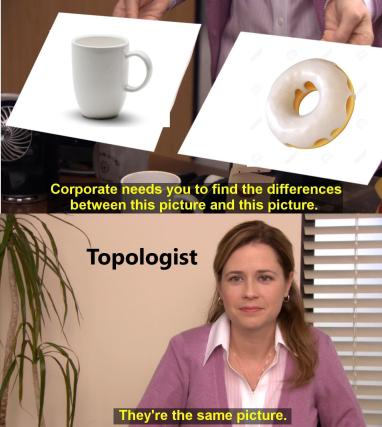
\includegraphics[scale=0.55]{geo.png}
    \vfill

    \vspace{0.8cm}

    \small
    Based on my understanding of lectures and notes of Prof Anrew Jay Lobb,
    based on notes by Prof Dirk Shutz\\
    
    \@date{}
  \end{center}
\end{titlepage}

\tableofcontents
\newpage

\begin{section}{Important Definisions}

  A place for short and important definisions \\
  \textsc{Definision} (Achiral) \textit{A link which is isotopic to its
    mirror image is called \textbf{achiral}.} \\
  \textsc{Definision} (Topological Invariant) \textit{It is a property of
    a \textbf{surface} which does not change under \textbf{homeomorphism}.} \\
  \textsc{Definision} (Isotopy Invariant for knots) \textit{Property which does
    not change under isotopy (mostly R-moves)}

\end{section}

\begin{section}{Basic Knot/Link Properties}

  \begin{subsection}{Tricolouring}
    Tricolouring can be used as one of the criteria to establish knot diagrams are different.
    This is invarient under all Reidemeister moves.

    Tricolouring rules:
    \begin{itemize}
      \item Each arc is assigned exacly one colour
      \item At least two colour are used
      \item At each crossing either 3 colours are used or only 1 colour is used
    \end{itemize}
    If all of these are met the diagram is called tricolourable.
  \end{subsection}

  \begin{subsection}{Writhe}
    Writhe of a knot diagram or an orientated link diagram D, mostly denoted as \(w(D)\),
    is a sum of all the positive crossings \(-\) the sum of all the negative crossings in D.
    Writhe of an orientated link diagram is dependent on the orientation of the link,
    and \emph{not invarient under R1 move}.
    Fromal definision is: \[w(D) = \sum_{x \in D} sign(x)\]
  \end{subsection}

\end{section}

\begin{section}{Knot/Link Polynomials}

  \begin{subsection}{Bracket Polynomial}

    Bracket Polynomial is a polynomial of an undirectd link in terms of A
    The bracket polynomial is invarient under R0, R2 and R3.
    Importantly bracket polynomial \emph{is not invarient under R1},
    \[\left\langle D \right\rangle = -A^{3n} \left\langle D' \right\rangle\]
    where D' is D after a R1 and \(n=1\) for positive R1 and \(n=-1\) for
    negative R1.

    This are the basic rules that establis how the bracket polynomials work:
    \begin{enumerate}
      \item \(\left\langle \Circle \right\rangle = 1\) where \(\Circle\) is the
            unknot
      \item \(\left\langle \Circle + D \right\rangle =- (A^{2} + A^{-2}) \left\langle D\right\rangle\)
            where D is any link diagram
      \item
            \(\left\langle \UCross \right\rangle = A \left\langle \RSmooth \right\rangle + A^{-1} \left\langle \LSmooth \right\rangle\)
    \end{enumerate}

    Bracket polynomials of some basic link diagrams:
    \begin{itemize}
      \item Trefoil \(= A^{-7} - A^{-3} - A^{-5}\)
      \item Figure8 \(= A^{-8} - A^{-4} + 1 - A^{4} + A^{8}\)
      \item Hopflink \(= -A^{-4} - A^{4}\)
    \end{itemize}

  \end{subsection}

  \begin{subsection}{X-Polynomial}
    
    The X-polynomial, denoted as \(X(D)\) or \(X(D)[A]\),
    is a development upon the bracket polynomial, now depending on the
    orientation of the link.
    This polynomial is in terms of A.
    This makes the X-polynomial \emph{invarient under all} Reidemeister moves.

    This is achived through: \[X(D) = (-A){}^{-3w(D)} \left\langle D \right\rangle\]
    where w is the writhe of D.

    A knot is called achiral if \(X(D)[A] = X(D)[A^{-1}]\).

  \end{subsection}

  \begin{subsection}{Jones Polynomial}

    The Jones polynomial, denoted as \(V_{D}(t)\), as is simply the X-polynomial
    with \(A = t^{-\frac{1}{4}}\), meaning it is definded as:
    \[V_{D}(t) = X(D)[t^{-\frac{1}{4}}]\]

  \end{subsection}

  \begin{subsection}{Alexander-Conway Polynomial}

    The Alexander-Conway polynomial, denoted \(\nabla_{K}(z)\)
    is another polynomial to express a knot or link diagram. It also acts on
    orientated link diagrams.
    There is no way to determin the achiral with this polynomial.

    \begin{itemize}
      \item \(K_{+} = K\) is the original link contatint a positive crossing
            \(\DPCross\)
      \item \(K_{-}\) is the link after changing the crossing to \(\DNCross\)
      \item \(K_{0}\) is the link after changing the crossing to \(\DSmooth\)
    \end{itemize}

    Rules for computing the Alexandr-Conway polynomial
    \begin{enumerate}
      \item \(\nabla_{U}(z) = 1\) where the U is the unknot
      \item \(\nabla_{K_{+}}(z) - \nabla_{K_{-}}(z) = z\nabla_{K_{0}}(z)\)
    \end{enumerate}

    Alexander-Conway polynomials of some basic link diagrams:
    \begin{itemize}
      \item \(\nabla_{U_{2}} = 0\)
      \item Hopflink \(= z\) with same orientation
      \item Hopflink \(= -z\) with different orientations
      \item Trefoil \(= z^{2} + 1\)
    \end{itemize}

  \end{subsection}

  \begin{subsection}{Absolute Polynomial}

    The absolute polynomial is the last polynomial tought on this course.
    It is expressed as \(Q_{L}(x)\) and does not take into account the orientation
    of the link diagram.

    \begin{itemize}
      \item \(L_{+}\) is the original containig \(\UCross\)
      \item \(L_{-}\) is the link after changing the crossing to \(\UOCross\)
      \item \(L_{0}\) is the link after changing the crossing to \(\RSmooth\)
      \item \(L_{\infty}\) is the link after changing the crossing to \(\LSmooth\)
    \end{itemize}
    \emph{Important note} both \(L_{+}\), \(L_{-}\) and  \(L_{0}\), \(L_{\infty}\)
    are interchangable!

    Rules for compuing the absolute polynomial
    \begin{enumerate}
      \item \(Q_{U}(x) = 1\) where U is the unknot
      \item \(Q_{L_{+}} + Q_{L_{-}} = x(Q_{L_{0}} + Q_{L_{\infty}})\)
    \end{enumerate}

    Absolute polynomials of some basic link diagrams:
    \begin{itemize}
      \item \(Q_{U_{2}} = 2x^{-1} - 1\)
      \item Hopflink \(= 2x + 1 + 2x^{-1}\)
      \item Trefoil \(= 2x^{2} + 2x - 3\)
    \end{itemize}

  \end{subsection}

\end{section}

\begin{section}{Surfaces}

  \begin{subsection}{Surface}

    Fistly defining \(D^{2}\). \[D^{2} = \{ (x, y) \in \mathbb{R}^{2} : x^{2} + y^{2} \leq 1 \}\]
    This means \(D^{2}\) is a \textbf{standard 2D} unit disc in \(\mathbb{R}^{2}\)
    with the origin at \textbf{0}. A surface is a object that looks like \(D^{2}\)
    localy. \[D(\textbf{p}; r) = \{ (x, y, z) \in \mathbb{R}^{3} :
      (x - p_{1})^{2} + (y - p_{2})^{2} + (z - p_{3})^{2} \leq r^{2} \}\]
    This ia a ball or radious r around point \textbf{p}.

    \textsc{Definision 2.1} (Surface) \textit{A \textbf{(parametric) surface S}
      in \(\mathbb{R}^{3}\) is a subset \(S \subset \mathbb{R}^{3}\) such that for
      every point \textbf{p} \(\in S\) there exists an injective, continously
      differentiable map \(\varphi: D^{2} \mapsto \mathbb{R}^{3}\)
      satisfying the following}:
    \begin{enumerate}
      \item \textit{We have \(\varphi(\textbf{0}) = \textbf{p}\)} and
            \(\varphi(D^{2}) = S \cap D(\textbf{p}, r)\) for some \(r > 0\)
      \item \textit{The matrix of partial derivatives}
            \textit{\[ D_{\varphi}(a, b) =
            \begin{pmatrix}
              \frac{\partial \varphi_{1}}{\partial x_{1}}(a, b) & \frac{\partial \varphi_{1}}{\partial x_{2}}(a, b) \\
              \frac{\partial \varphi_{2}}{\partial x_{1}}(a, b) & \frac{\partial \varphi_{2}}{\partial x_{2}}(a, b) \\
              \frac{\partial \varphi_{3}}{\partial x_{1}}(a, b) & \frac{\partial \varphi_{3}}{\partial x_{2}}(a, b)
            \end{pmatrix}\]}
            \textit{has rank 2 for every \((a, b) \in D^{2}\)}
    \end{enumerate}
    \textit{Where
      \(\varphi(x, y) = (\varphi_{1}(x, y), \varphi_{2}(x, y), \varphi_{3}(x, y))\)
      and such a map is called a \textbf{parametrization around p} \(\in S\).}

    This means for each point \(\textbf{p} \in S\) there exists a map mapping
    all points from a disc around it to either the surface around (S) or a
    small ball around it (radius r). (Prey this is correct)

    If S is a surface and \(\textbf{p} \in S\), then \(S \backslash{}
    \{{} \textbf{p} \}{}\) is also a surface.

    A \textbf{surface} is called \textbf{compact} if it can be
    \textbf{triangulated}.
    It is also called \textbf{connected} if any two 0-simplexes can be joined by
    a finite amount of 1-simplexes in C.

    \emph{For a \textbf{compact surface} S and \(C_{1}, C_{2}\) \textbf{simplicial
        complexes} triangulating S. Then \(\chi(C_{1}) = \chi(C_{2})\).} This
    enables the notion of \textbf{Euler Characteristic} of a surface, \(\chi(S)\)
    which is equall to any C simplicial complex.

    A surface \(S \subset \mathbb{R}^{3}\) is uniquely determined
    (up to a homeomorphism) by
    \begin{itemize}
      \item Orientability
      \item Number of boundary circles
      \item Euler Characteristic
    \end{itemize}
    This is called the \textbf{classification theorem}.

  \end{subsection}

  \begin{subsection}{Surface with Boundary}

    A \textbf{surface with boundary} is a subset \(S \subset \mathbb{R}^{3}\)
    where for every point \(\textbf{p} \in S \; r > 0\) s.t.
    \(S \cap D(\textbf{p}; r)\) looks like \(D^{2}\) or its positive half.
    Looks likes means there is a \textbf{continously differentiable} map
    \(\varphi: X \to \mathbb{R}^{3}\) where \(X \in \{ D^{2}, D^{2}_{+} \}\).
    This map has to satisfy the first two conditions from the definision of a
    surface above.

    The \textbf{boundary} of such surface S, denoted \(\partial S\), consists of
    points \(\textbf{p} \in S\) for which \(\varphi(0) = \textbf{p}\) and
    \(\varphi(D^{2}_{+}) = S \cup D(\textbf{p}; r)\) for some \(r > 0\).
    Points in S which are not boundary, \(S/\partial S\), are called the
    \textbf{internal} points.

    For S a compact surface with boundary let C triangulate S. Then if
    \(\partial S \neq \emptyset\), it can be traiangulated by \(K \subset C\)
    with K only consisting of 1-simplexes. \emph{This implies the boundary is
    a link or a knot!}

  \end{subsection}

  \begin{subsection}{Seifert Surface}

    Every knot can be the boundary of an orientable surface. Such surface is
    called seifert surface.
    This is done by the following procedure:
    \begin{enumerate}
      \item Take knot D
      \item Smooth all edges similarly to Alexander polynomial
      \item Assgin opposite colours based on the orientation
      \item Re-introduce the crossing by a twisted rectangle
    \end{enumerate}

    \emph{These are always orientable} \\
    For such surface the genus \(g = \frac{1}{2} (k - s  + 1)\) where k is the
    number of crossings in the knot and s is the number of circles after smoothing.

    \emph{This surfaces are not unique, differnt surfaces can be bounded by the
      same knot and different knots can bound the same surface}


    Genus of a knot is definded to be the smallest \(g \geq 0\) that can be
    obtained by the formula above for the knot. This is isotopy invariance for
    knots. This is denoted as \(g(D)\). \\
    If \(g(D) = 0\) then D is the unkont. Genus of trefoil and figure-8 are both 1.
    For knots \(K_{1}, K_{2} \; g(K_{1} + K_{2}) = g(K_{1}) + g(K_{2})\). As
    \(g(D) \geq 0\) there are no additive inverses. Any knot K for which \(g(K) = 1\)
    is called prime. Any orientable knot can be factored into finite amount of prime
    knots. This factorisation is unique.

  \end{subsection}

  \begin{subsection}{Orientability}

    A surface S is called \textbf{orientable} if it has two sides, and
    the sides cannot be traveled in between without crossing a boundary.

    This can be determined by trying to colour a surface with two colours.

  \end{subsection}

  \begin{subsection}{Topological Invariant}

    Surfaces \(S_{1}, S_{2}\) are said to be \textbf{equivalent}, denoted as
    \(S_{1} \approx S_{2}\), if there exists a \textbf{continuous bijective}
    map \(f: S_{1} \to S_{2}\) such that \(f^{-1}: S_{2} \to S_{1}\) is also
    \textbf{continous}. The map f is called a \textbf{homeomorphism}.
    \emph{This equivalents is very weak.} The only requirement for this is
    for points that are close together to stay close together.

    Some examples of \textbf{topological invariants}
    \begin{itemize}
      \item \textbf{Compactness}
            Generalisation of close-and-bounded interval in \(\mathbb{R}\)
      \item \textbf{Connectedness}
            Is surface made from one or multiple `piece'
      \item \textbf{Genus}
            Number of `holes'
    \end{itemize}

    List of shapes \textbf{genus} of \(0 \dots \infty\) contains all shapes
    up to \textbf{orientability}.

    For a compact surfaces \(S_{1}, S_{2}\) and \(S_{1} \approx S_{2}\) then
    \(\chi(S_{1}) = \chi(S_{2})\).

  \end{subsection}

  \begin{subsection}{Simplexes}

    For a list of \(k + 1\) points \(\textbf{v}_{0}, \dots , \textbf{v}_{k} \in \mathbb{R}^{n}\)
    where \(v_{i} = \{ (x_{1}, \dots , x_{n}) | x_{j} \in \mathbb{R} \}\) for all i.
    The \textbf{convex hull} of these points, denoted \(c(\textbf{v}_{0}, \dots , \textbf{v}_{k})\) is
    \(c(\textbf{v}_{0}, \dots , \textbf{v}_{k}) = \sum_{i = 0}^{k}\lambda_{i}v_{i} \in \mathbb{R}\)
    where all \(\lambda \in [0, 1]\) and \(\sum_{i = 0}^{k}\lambda_{i} = 1\). \\
    We say \(\textbf{v}_{0}, \dots , \textbf{v}_{k}\) are in \textbf{general position} if
    \(\textbf{v}_{1} - \textbf{v}_{0}, \dots , \textbf{v}_{k} - \textbf{v}_{0}\)
    are all \textbf{linearly independent}. In that case their \textbf{convex hull}
    of these points is a k-dimensional object.

    A \textbf{k-simplex} is the \textbf{convex hull} of \(k + 1\) of points
    \(\textbf{v}_{0}, \dots , \textbf{v}_{k}\) in \textbf{general position}.
    These points \textbf{span} the simplex. \\
    If \(\textbf{v}_{0}, \dots , \textbf{v}_{k}\) is a k-simplex then for
    \(\{ i_{0}, \dots , i_{r} \} \subset \{ 0, \dots , k \}\) then
    \(\textbf{v}_{i_{0}}, \dots , \textbf{v}_{i_{r}}\) spans some r-simplex and
    \(c(\textbf{v}_{i_{0}}, \dots , \textbf{v}_{i_{r}}) \subset
    c(\textbf{v}_{0}, \dots , \textbf{v}_{k})\), and it is called a \textbf{sub-simplex}. \\
    In general any sub-simplex will be called \textbf{r-face} of the original simplex. \\
    A \((k - 1)\)-face is called a \textbf{proper face}.

    A finite collection C of \textbf{simplexes} in \(\mathbb{R}^{n}\) is called
    a \textbf{simplicial complex } if
    \begin{itemize}
      \item if \(\sigma \in C\) and \(\tau \leq \sigma\) then \(\tau \in C\)
      \item For \(\sigma_{1}, \sigma_{2} \in C\) if
            \(\sigma_{1} \bigcap \sigma_{2} \neq \emptyset\) then
            \(\exists \tau \leq \sigma_{1}, \sigma_{2}\) s.t.
            \(\sigma_{1} \bigcap \sigma_{2} = \tau\)
    \end{itemize}
    Where for simplexes \(\tau, \sigma \; \tau \leq \sigma\) means \(\tau\)
    is a point/face/\dots contained in \(\sigma\). \\
    The dimention of C is the size of the biggest k-simplex. \\
    \(|C| \subset \mathbb{R}^{n}\) is called \textbf{polyhedron associated} to C.
    It is also often refered to as \textbf{triangle mesh}. It is defined to be
    \(|C| = \cup_{\sigma \in C} (\sigma)\).
    \emph{The polyhedron is not a surface as no differentiable parametrization
      is possible at the verticies.}

  \end{subsection}

  \begin{subsection}{Triangulation}

    A \textbf{triangulation} of a subset \(X \subset \mathbb{R}^{n}\) consists
    of a \textbf{simplicial complex} C and a \textbf{bijective continous} map
    \(h: |C| \to X\). It is said X is triangulated by C.

  \end{subsection}

  \begin{subsection}{Euler Characteristic}

    \textbf{Euler Characteristic}, denoted as \(\chi(C)\), with C a simplicial
    complex is defined to be \(\chi(C) = \sum_{i = 0}^{\infty} (-1)^{i}a_{i}(C)\)
    where \(a_{i}(C)\) is the number of i-simplexes in C.

    For \(S_{1}, S_{2}\) compact surfaces if \(S_{1} \approx S_{2}\) then
    \(\chi(S_{1}) = \chi(S_{2})\).
    For a surface S of \textbf{genus} g, denoted \(S_{g}\), with \(g \geq 0\)
    then \(\chi(S_{g}) = 2 - 2g\). \\
    This can be used to redefined \textbf{genus} of surface S to be
    \(g = 1 - \frac{\chi(S)}{2}\). If d discs are removed from S and S is
    orientable then \(\chi(S_{d}) = 2 - 2g -d\).

    Euler characteristic of a disc is +1 and for a rectangle it is also +1
    but if the rectangle is attached it is -1 per side attached. This usually
    results in the rectangle being -1.

  \end{subsection}

\end{section}

\begin{section}{Differential Topology}

  \begin{subsection}{Basic maps}

    Unit circle \(S^{1} := \{ z \in \mathbb{C} \; | \; |z| = 1 \}\). \\
    The exponential map \(e: \mathbb{R} \to S^{1}\) is \(e(t) = e^{w\pi{}it}\).
    This is continous and surjective. As t increases output moves around \(S^{1}\)
    anticlockwise with unit direction. To go the opposite direction -t should be used.

    Every continous map \(\lambda : S^{1} \to S^{1}\) has a function
    \(\tilde\lambda : \mathbb{R} \to \mathbb{R}\) with
    \[e(\tilde\lambda(t)) = \lambda(e(t)).\] This \(\tilde\lambda\) is called
    \textbf{lift} of \(\lambda\). This is not unique.
    But \(w = \tilde\lambda(1) - \tilde\lambda(0)\) is only dependednt on \(\lambda\),
    and \(w \in \mathbb{Z}\) for all \(\lambda\).

    Two continous maps \(\lambda_{0}, \lambda_{1} : S^{1} \to S^{1}\) are called
    \textbf{homotopic} if there exists a map \(H: S^{1} \times [0, 1] \to S^{1}\)
    s.t. \(H(z, 0) = \lambda_{0}(z)\) and \(H(z, 1) = \lambda_{1}(z) \;
    \forall z \in S^{1}\). This is true if \(\omega(\lambda_{1}) = \omega(\lambda_{2})\).

  \end{subsection}

  \begin{subsection}{Winding number}

    For any \(\lambda : S^{1} \to S^{1}\) the functoin
    \(\omega(\lambda) := \tilde\lambda(1) - \tilde\lambda(0)\). As said above it
    does not depend on the choice of \(\tilde\lambda\) and it is always
    positive. For multiplication of two maps \(\lambda_{1}, \lambda_{2}\)
    the winding number is added.

  \end{subsection}

  \begin{subsection}{Extension to non Unit Circles}

    For a function \(p(z) = a_{n}z^{n} + a_{n - 1}z^{n - 1} + \dots + a_{1}z + a_{0}\)
    for \(z \in \mathbb{C}\), if \(p(z) \neq 0 \; \forall z \in S^{1}\) then
    \(\lambda_{p}(z) := \frac{p(z)}{|p(z)|}\), with a \textbf{winding number}
    \(\omega(\lambda_{p})\).

  \end{subsection}

  \begin{subsection}{Vector Fields}

    For \(\mathbb{R}^{2} = \{ (x, y) : x, y \in \mathbb{R} \}\) and equivalents
    in \(\mathbb{C}\) where \(c = x + iy\). For \(z \in \mathbb{C}\) and \(r > 0\)
    \(D(z; r) := \{ w \in \mathbb{C} : |z - w| \leq r \}\) is a closed disc around
    point z with radious r.

    \(U \subset \mathbb{C}\) is called a \textbf{region} if \(U \neq \emptyset\)
    and \(\forall z \in U \exists r > 0\) s.t. \(D(z; r) \subset U\). This means
    for each point in U all points in an infinitely small circle around are
    also in U.

    For \(U \in \mathbb{C}\) a region, a \textbf{vector field on U} is a
    \textbf{continously differentiable function} \(v: U \to \mathbb{R} = \mathbb{C}\).
    \emph{It has to be differentiable in real numbers.} \(v(z)\) is a vector based
    at point \(z \in U\), meaning for every point (or complex number) \(z \in U\)
    there is another vector (also complex number) attached to z. \\

  \end{subsection}

  \begin{subsection}{Singularity}

    A \textbf{singularity} of v is a point \(p \in U\) with \(v(p) = 0\).
    It is called \textbf{isolated} if \(\exists r > 0\) s.t. \(D(p; r) \subset U\)
    and \(v(q) \neq 0 \; \forall q \in D(p; r), q \neq p\). Meaning there is no other
    point in an infinitely small disc around the \textbf{singularity} that is also
    a \textbf{singularity}.
    The boundry of this disc can be written as \(\partial D(p; r) =
    \{ p + rz : z \in  S^{1} \}\). \\
    A map \(\lambda_{r} : S^{1} \to S^{1}\) is defined as \(\lambda_{r}(z) =
    \frac{v(p + rz)}{|v(p + rz)|}\). This function takes a value at the edge
    of the disc and scale them to unit vectors.

    \textbf{Index} of an \textbf{isolated singularity} \(p \in U\) of v,
    denoted as \(I(p)\), is defined to be \(I(p) = \omega(\lambda_{r})\) with r
    the radious of the disc of no singularities around p. As \(\omega(\lambda_{r})
    = \omega(\lambda_{r'})\) the index is not dependent on r. This means it usually
    is best to use \(r = 1\).

  \end{subsection}

  \begin{subsection}{Tangent Curves}

    Every vector field \(v: U \to \mathbb{C} = \mathbb{R}^{2}\) determines a
    differential equation \(\delta'(t) = v(\delta(t))\) with \(\delta(0) = z_{0}
    \in U\). Given an \(z_{0} \in U\) there is a \textbf{unique} curve \(\delta_{z_{0}}
    : (a, b) \to U\) which solves the initial value problem with \(a < 0 < b\).

    For any singularity p \(\delta_{p}(t) = p\) provides a solution to the
    differential equation above. For every \(z_{0} \in U\) not a singularity
    \(\delta_{z_{0}}\) is a curve in U. These solutions are called \textbf{tangental
      curves} of the vector field v. This curves always begin and end at
    singularities or approaching boundary of U.

    For a disc \(D^{2} = \{ (x, y) \in \mathbb{R} : x^{2} + y^{2} \leq 1\}\)
    with finitely many singularities \(\omega(\lambda) = \sum^{k}_{i = 1}I(p_{i})\)
    where all \(p_{i}\)s are singularities.

  \end{subsection}

  \begin{subsection}{A useful fact?}

    For \(\cdot\) representing vector dot product, for a vector field v defined
    on \(D^{2}\) if \(\forall z \in S^{1} \; v(z) \cdot z > 0\) then v contains
    at least one singularity. Furthermore if v has finitely many singularities
    then the sum of the indexes is 1 if \(v(z) \times z > 0\) for all z.

  \end{subsection}

  \begin{subsection}{Vector Fields on Surfaces}

    For S a surface, no matter the boundary, a vector \(v \in \mathbb{R}^{3}\)
    is called a \textbf{tangent vector} to \(p \in S\) if \(\exists \phi_{p}
    : (-\epsilon, \epsilon) \to \mathbb{R}^{3}\) with
    \begin{itemize}
      \item \(\phi_{p}\) is continously differentiable
      \item \(\phi_{p}(0) = p\)
      \item \(\phi'_{p}(0) = v\)
      \item if \(p \notin \partial S\) then \(\phi_{p}(t) \in S \;
            \forall t \in (-\epsilon,\epsilon)\)
      \item if \(p \in \partial S\) then \(\phi_{p}(t) \;
            \forall t \in (-\epsilon, 0] \cup [0, \epsilon)\)
    \end{itemize}
    The last two points can be summerised to say \(\phi_{p}\) maps all \(t \neq 0\)
    to inside S.

    A continously differentiable map \(v: S \to R^{3}\) is called a \textbf{vector field}
    on S if \(v(p)\) is a \textbf{tangent vector} to p \(\forall p \in S\). A
    singularity of v can be defined similarly to the one for regular vecotr fields. \\
    A simpler condition for a \textbf{vector field} \(v: S^{2} \to \mathbb{R}^{3}\)
    iff \(v(p) \cdot p = 0 \; \forall p \in S^{2}\). No idea why \(S^{2}\) not S.

    Given a vector field v on S, it can be \textit{pulled back} from around any
    \(p \in S\) to a vector field w on \(D^{2}\) s.t.\ for every \(z \in D^{2}\)
    \(D_{\varphi_{p}}(z)w(z) = v(\varphi_{p}(z))\). \\
    \(D_{\varphi_{p}}(\textbf{0})\) is an injective linear map so if p is an
    isolated singularity of v, then \(D_{\varphi_{p}}(\textbf{0})w(\textbf{0}) = 0\).
    This implies \(w(\textbf{0}) = \textbf{0}\). This means \(\textbf{0}\) is an
    isolated singularity of w. This does not depend on the parametrization.


  \end{subsection}

  \begin{subsection}{Index on Surfaces}

    For \(p \in S\) an isolated singularity of a vector field v on a surface
    S, with \(p \notin \partial S\), index of p, denoted \(I(p)\), is deined to be
    \(I(\textbf{0})\) where \textbf{0} is the corresponding isolated singularity
    on the \textit{pulled-back} vector field.

    A vector field on \(S^{2}\) must have a singularity, and if it has finitely
    many singularities the sum of their indecies is equal to 2.

    For \(S \subset \mathbb{R}^{3}\) a \textbf{compact, connected and orientable}
    surface, no matter the boundary and \(v: S \to \mathbb{R}^{3}\) a vector
    field with finitely many singularities \(p_{1} \dots p_{m}\). Assume v points
    towards a boundary, then \(\sum^{m}_{i = 1} I(p_{i}) = \chi(S)\). \\
    This holds for all connected components of a not connected surface.

  \end{subsection}

\end{section}

\end{document}
